% !TEX TS-program = pdflatex
% !TEX encoding = UTF-8 Unicode

% This is a simple template for a LaTeX document using the "article" class.
% See "book", "report", "letter" for other types of document.

\documentclass[11pt]{article} % use larger type; default would be 10pt

\usepackage[utf8]{inputenc} % set input encoding (not needed with XeLaTeX)

%%% Examples of Article customizations
% These packages are optional, depending whether you want the features they provide.
% See the LaTeX Companion or other references for full information.

%%% PAGE DIMENSIONS
\usepackage{geometry} % to change the page dimensions
\geometry{a4paper} % or letterpaper (US) or a5paper or....
% \geometry{margin=2in} % for example, change the margins to 2 inches all round
% \geometry{landscape} % set up the page for landscape
%   read geometry.pdf for detailed page layout information

\usepackage{graphicx} % support the \includegraphics command and options

% \usepackage[parfill]{parskip} % Activate to begin paragraphs with an empty line rather than an indent

%%% PACKAGES
\usepackage{booktabs} % for much better looking tables
\usepackage{array} % for better arrays (eg matrices) in maths
\usepackage{paralist} % very flexible & customisable lists (eg. enumerate/itemize, etc.)
\usepackage{verbatim} % adds environment for commenting out blocks of text & for better verbatim
\usepackage{subfig} % make it possible to include more than one captioned figure/table in a single float
% These packages are all incorporated in the memoir class to one degree or another...
\usepackage{enumitem}
\usepackage{hyperref}
\usepackage{tikz}
\usetikzlibrary{backgrounds, positioning, shapes.geometric}
\usepackage{xcolor}

\hypersetup{
    colorlinks=true,
    linkcolor=red,
    filecolor=red,      
    urlcolor=red,
    pdfpagemode=FullScreen,
    }
\urlstyle{same}

%%% HEADERS & FOOTERS
\usepackage{fancyhdr} % This should be set AFTER setting up the page geometry
\pagestyle{fancy} % options: empty , plain , fancy
\renewcommand{\headrulewidth}{0pt} % customise the layout...
\lhead{}\chead{}\rhead{}
\lfoot{}\cfoot{\thepage}\rfoot{}

%%% SECTION TITLE APPEARANCE
\usepackage{sectsty}
\allsectionsfont{\sffamily\mdseries\upshape} % (See the fntguide.pdf for font help)
% (This matches ConTeXt defaults)

%%% ToC (table of contents) APPEARANCE
\usepackage[nottoc,notlof,notlot]{tocbibind} % Put the bibliography in the ToC
\usepackage[titles,subfigure]{tocloft} % Alter the style of the Table of Contents
\renewcommand{\cftsecfont}{\rmfamily\mdseries\upshape}
\renewcommand{\cftsecpagefont}{\rmfamily\mdseries\upshape} % No bold!

%%% END Article customizations

%%% The "real" document content comes below...

\title{Chapter 1}
\date{} % Activate to display a given date or no date (if empty),
         % otherwise the current date is printed 

\begin{document}
\maketitle

\section*{Creating Your First Unreal C++ Game}

\textbf{Unreal Engine (UE)} is one of the most popular 3D computer graphics game engines developed by Epic Games, providing a comprehensive set of tools and functionalities to develop high-quality, immersive 3D simulations. The engine offers its intuitive visual scripting system, \textbf{Blueprint}, and a robust \textbf{C++} programming framework for developers of all skill levels. This book provides a concise introduction to C++ programming and demonstrates how to write C++ scripts in UE for game development.

In this chapter, you will learn the essential skill of creating an Unreal C++ project from scratch or converting an existing Unreal Blueprint project into an Unreal C++ project, which serves as a fundamental skill to advance in game development. By mastering this process, you will gain the necessary foundation to take your game development abilities to the next level.


This chapter will cover the following topics:

\begin{itemize}
	\item Understanding C++ scripting in Unreal
	\item Creating your C++ shooter project from a template
	\item Converting an existing Blueprint project to a C++ project
\end{itemize}

\subsection*{Technical Requirements}

As a reader of this book, you will be expected to have common computer operational skills. You should also have basic knowledge of and experience with the UE5 editor, as well as some Blueprint scripting skills.

To follow this chapter, you should have installed Epic Games Hub and the 5.03 or later version of the engine editor on your computer. If you haven’t done so, please go to the official Epic website (\url{https://www.unrealengine.com/en-US}) to register an account and download the Epic Games Launcher.

The minimum required development environment is as follows:

\begin{itemize}
\item \textbf{Operating system}: Windows 10
\item \textbf{Processor}: Intel 7th generation or equivalent
\item \textbf{Memory}: 16 GB of RAM
\item \textbf{GPU}: GTX 1080 (or AMD equivalent)
\item \textbf{DirectX}: Version 12
\item \textbf{Storage}: 25 GB of available space
\item \textbf{Additional notes}: 8 GB of VRAM recommended
\end{itemize}

The official system requirements can be found here: \url{https://docs.unrealengine.com/5.0/en-US/hardware-and-software-specifications-for-unreal-engine/}. To save game editing time in the UE5 editor, it is recommended to use a computer with an i9 (or an AMD equivalent) CPU, 64 GB of RAM, and a GeForce RTX 3060 video card.

\subsection*{Understanding C++ scripting in Unreal}

Before getting started, we need to answer some questions that people usually ask about \textbf{C++ scripting}. This will help to clarify the pros and cons of using C++, the reasons to use C++, and the difference between UE C++ scripting and C++ programming.

\subsubsection*{What is the difference between C++ and Blueprint?}

Both C++ and Blueprint are scripting languages that can accomplish the same tasks, but one might be better suited than the other under certain circumstances. The main difference between them is that C++ is a programming language that allows you to write general-purpose, text-based code, whereas Blueprint is a visual scripting system for UE.

For UE projects, game studios usually use both C++ and Blueprint to develop commercial-level games. C++ is usually used for advanced techniques, complex algorithms, and big-scale logic code. If you can script with C++, you will have more chances to work on a professional team.

One of the most important advantages of using C++ is performance. C++ allows you to write low-level operational code. It also provides control over the core system that is not accessible to Blueprint. In addition, the final C++ code will eventually be optimized and compiled to be machine-friendly binary native code. On the other hand, Blueprint scripts are interpreted and executed by a middle layer, which means more execution time.

C++ code and files can be well-organized based on an entire project’s mechanics. It is easy to globally search, locate, and access code blocks to edit, maintain, and troubleshoot. In the meantime, it is also easier to read and understand a big chunk of code that implements complex algorithms and logic. Blueprint, on the other hand, is a context-sensitive scripting environment. Blueprint graphs are relatively independent. When a graph needs to solve complex logic, the nodes and the connection lines create messy spaghetti that can hardly be understood and maintained.

C++ also has some shortcomings. One example is that it may cause critical errors that may crash an entire system. That is usually caused by the developer’s mistakes. Since Blueprint is a protected layer, it is safer, and hence, the chances of the system crashing are fewer.

In conclusion, the choice between C++ and Blueprint should be made based on specific development requirements and conditions, considering the pros and cons of each approach.

\subsubsection*{When do you use C++?}

Both C++ and Blueprint can handle game development processes without a problem. There is no exact rule that regulates when to use C++ or Blueprint. It mainly depends on your experience and the actual needs of different games. You make your own decision based on how much you know about the two scripting systems.

Before you start working on something, you can ask yourself this question: “Where does it make sense to use C++, and where does it make sense to use Blueprints?” We recommend basing your answer on the following aspects and trade-offs:

\begin{itemize}
\item Performance
\item Logic and algorithm complexity
\item Accessibility to a system’s core functions
\item The developer’s experience
\end{itemize}

If you want higher performance and deal with advanced game logic and system processes, and you are capable of coding and solving complex problems, you should go for C++.

\subsubsection*{What is tje difference between C++ programming and C++ scripting?}

You may be confused about the difference between C++ programming and C++ scripting. We want to clarify the meanings of these two terms.

C++ programming means using the C++ programming language to write code for any purpose; it doesn’t have to be just for UE projects. C++ scripting, in this book, is a specific dialect of the C++ programming language supported by the UE. It takes advantage of the power of C++ syntax and also works with UE’s \textbf{Application Programming Interfaces (APIs)}, which allow developers to create and extend the engine’s functionalities for their games and the development environment’s context, such as objects, graphics, audio, and network communication.

Now that we have a basic overview of C++ and have learned why and when to use C++ for Unreal game developments, let’s dive deeper into C++ scripting by creating a sample project.

\section*{Creating your C++ Shooter project from a template}

Now, it’s the time to get your hands dirty working on a UE5 C++ project yourself. We will go through the steps to create a new C++ project from scratch based on the \textbf{First Person} template.

The \textbf{First Person} template is one of the default game templates that come with UE. When you want to create a new project, you can pick this template from the \textbf{Unreal Project Browser} window. Our new MyShooter game will derive all the features from the template game, and we don’t have to do any additional work.

To get started with C++ scripting, we first need to install an IDE. In this book, we will use MS Visual Studio 2022 as an example.

\subsubsection*{Installing Visual Studio 2022}

\textbf{Visual Studio (VS)} is an \textbf{Integrated Development Environment (IDE)} from Microsoft. It is a tool used to create, edit, debug, and compile code. In order to do C++ scripting, you need to go to the official website at \url{https://visualstudio.microsoft.com/vs/} and download the \textbf{Community 2022} version installation package (see Figure 1.1).

\begin{center}
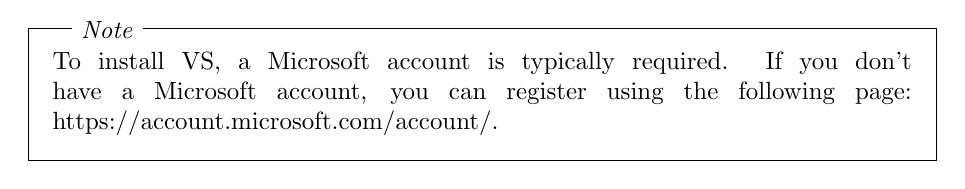
\begin{tikzpicture}[show background rectangle, scale=0.9, every node/.style={scale=0.9}]
\node[align=justify, text width=\textwidth, inner sep=0.5em]{
To install VS, a Microsoft account is typically required. If you don’t have a Microsoft account, you can register using the following page: https://account.microsoft.com/account/.
};
\node[xshift=3ex, yshift=-0.7ex, overlay, fill=white, draw=white, above right] at (current bounding box.north west) {\textit{Note}};
\end{tikzpicture}
\end{center}

Next, launch \textbf{VisualStudioSetup.exe} inside the folder where you downloaded the VS installer (the \textbf{Downloads} folder, for example).

Enable the two \textbf{Game development with C++} and \textbf{Desktop development with C++} checkboxes – these two options tell the installer to install the C++ compiler and the professional game development support for UE.

Also, keep an eye on the following options on the \textbf{Installation details} panel that belongs to the \textbf{Desktop development with C++} group, and make sure the following are checked:

\begin{itemize}
\item C++ profiling tools
\item C++ AddressSanitizer
\item Windows 10 SDK
\item IntelliCode
\item IDE support for Unreal Engine
\end{itemize}

Then, click the \textbf{Install} button to install the workloads and reboot the system, and then you will see a prompt from the dialog popup.

The next thing we need to do is to confirm that we have installed the engine source code together with the UE5 editor. The reason why we need this is that when we generate a new project, the engine source code can be integrated into the new project; under certain circumstances, we may need to modify or customize the engine for the game’s specific needs.

\subsubsection*{Ensuring your UE has the source code installed}

Before launching the UE5 editor, we first need to check whether \textbf{Engine Source} is installed for the editor. By doing this check, we make sure that the UE5 source code is integrated with the C++ projects we are going to create.

The three steps to check or install the engine source code are as follows:

\begin{itemize}
\item Click the downward arrow button and choose Options from the drop-down menu.
\item Make sure that the \textbf{Engine Source} option is checked.
\item Press the \textbf{Apply} button
\end{itemize}

UE is an ongoing development product, with bugs and defects that may need to be fixed by its users. Also, professional developers sometimes modify the engine source code to adapt to their specific needs. An example of this is when we face an issue with geometry instancing (or instanced rendering) working only in the game’s development build but not in the release build, which is subsequently resolved by our engineer modifying the engine’s source code.

\begin{center}
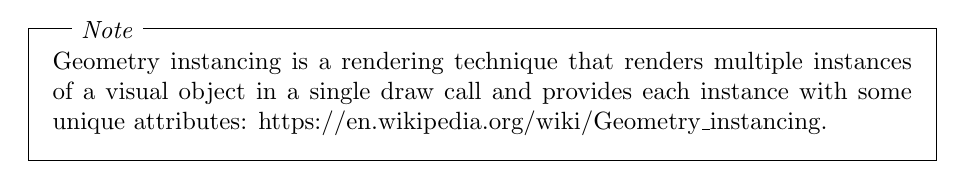
\begin{tikzpicture}[show background rectangle, scale=0.9, every node/.style={scale=0.9}]
\node[align=justify, text width=\textwidth, inner sep=0.5em]{
Geometry instancing is a rendering technique that renders multiple instances of a visual object in a single draw call and provides each instance with some unique attributes: https://en.wikipedia.org/wiki/Geometry\_instancing.
};
\node[xshift=3ex, yshift=-0.7ex, overlay, fill=white, draw=white, above right] at (current bounding box.north west) {\textit{Note}};
\end{tikzpicture}
\end{center}

We are now ready to start the UE editor through the Epic Games Launcher.

\subsubsection*{Launching the UE5 editor through the Epic Game Launcher}

Launching the UE5 editor is pretty straightforward. You simply click the \textbf{Launch} button on the 5.03 engine card to start the editor.

The next thing we want to do is to create a new game project. Let’s name the new project \textbf{MyShooter}.

\subsubsection*{Creating the MyShooter C++ project}

To create the project, follow these steps:

\begin{itemize}
\item In the \textbf{Unreal Project Browser} window, choose the \textbf{GAMES} tab on the left side.
\item Select the \textbf{First Person} template.
\item Select the \textbf{C++} button.
\item Choose the project location (for example, \textbf{C:\\UEProjects}) and type \textbf{MyShooter} in the Project Name field.
\item Click the Create button.
\end{itemize}

The created game project also includes the starter content, which is packaged with assets and resources that can be used to prototype the game.

The engine will do some initialization work and then open the editor when things are ready. If you look at the project tree panel’s \textbf{MyShooter} tab in the bottom-left corner of the editor window, you should see the \textbf{C++ Classes} node on the same layer as the Content node.

\subsubsection*{Associating VS with UE5 as the default source code editor}

Since we created the C++, project, all the C++ source code for the game was already generated. To open the source files directly in the UE5 editor, we want to associate VS as the engine editor’s default IDE.

On the UE5 Editor’s main menu, select \textbf{Edit | Editor Preferences} to open the preference window, then find the \textbf{General | Source Code} item on the left panel, and finally, pick \textbf{Visual Studio 2022} from the \textbf{Source Code Editor} dropdown.

You can now use VS to open the source code files.

\subsubsection*{Opening the C++ source code in VS (optional)}

If you want to open and view the C++ source code in VS, you can find the source code file (for example, \textbf{C++/MyShooter/MyShooterCharacter.cpp}) in the project and simply double-click on it. The system will automatically launch VS, and the VS editor will open the \textbf{MyShooterCharacter.cpp} file.

Back in the Unreal editor, click the \textbf{Play} button to start the game. While playing the game on the battlefield, you can control your character, move them around, and pick up the gun in front of them.

We have learned how to create a \textbf{UE} C++ project from scratch. However, what if we already have a Blueprint project and want to convert it to a C++ project? UE allows developers to do it by adding a new C++ class to the project. Let’s practice converting a MyBPShooter Blueprint project.

\subsubsection*{Converting an existing Blueprint project to a C++ project}

UE provides a very straightforward way to convert an existing Blueprint project to a C++ project. All you need to do is add a C++ class to your project and then let UE take care of the conversion and add the needed project files:

\begin{itemize}
\item First of all, you have to create a Blueprint project, \textit{MyBPShoopter}, under \textbf{C:\\UEProjects} (you can choose a different path to create the new project). Use the same steps introduced in the \textit{Creating the MyShooter C++ project} section, but choose \textbf{BLUEPRINT} instead of \textbf{C++} for the creation of the \textit{MyBPShooter} project.


\end{document}
